\documentclass{slide}
\usepackage{tikz}

\usetikzlibrary{arrows}

\usepackage{tabto}

\usepackage{languages}

% \usepackage{pgfpages}
% \setbeameroption{show notes on second screen}

\title{Distributed Computing II}
\subtitle{CSSE6400}
\author{Brae Webb}
\date{\week{6}}

% \titlegraphic {
%     \tweet%
%     {images/mathiasverraes}%
%     {Mathias Verras}%
%     {mathiasverraes}%
%     {There are only two hard problems in distributed systems:  2. Exactly-once delivery 1. Guaranteed order of messages 2. Exactly-once delivery}%
%     {https://twitter.com/mathiasverraes/status/632260618599403520}%
% }

\begin{document}

\maketitle

\point[Previously in CSSE6400\dots]{
\begin{center}
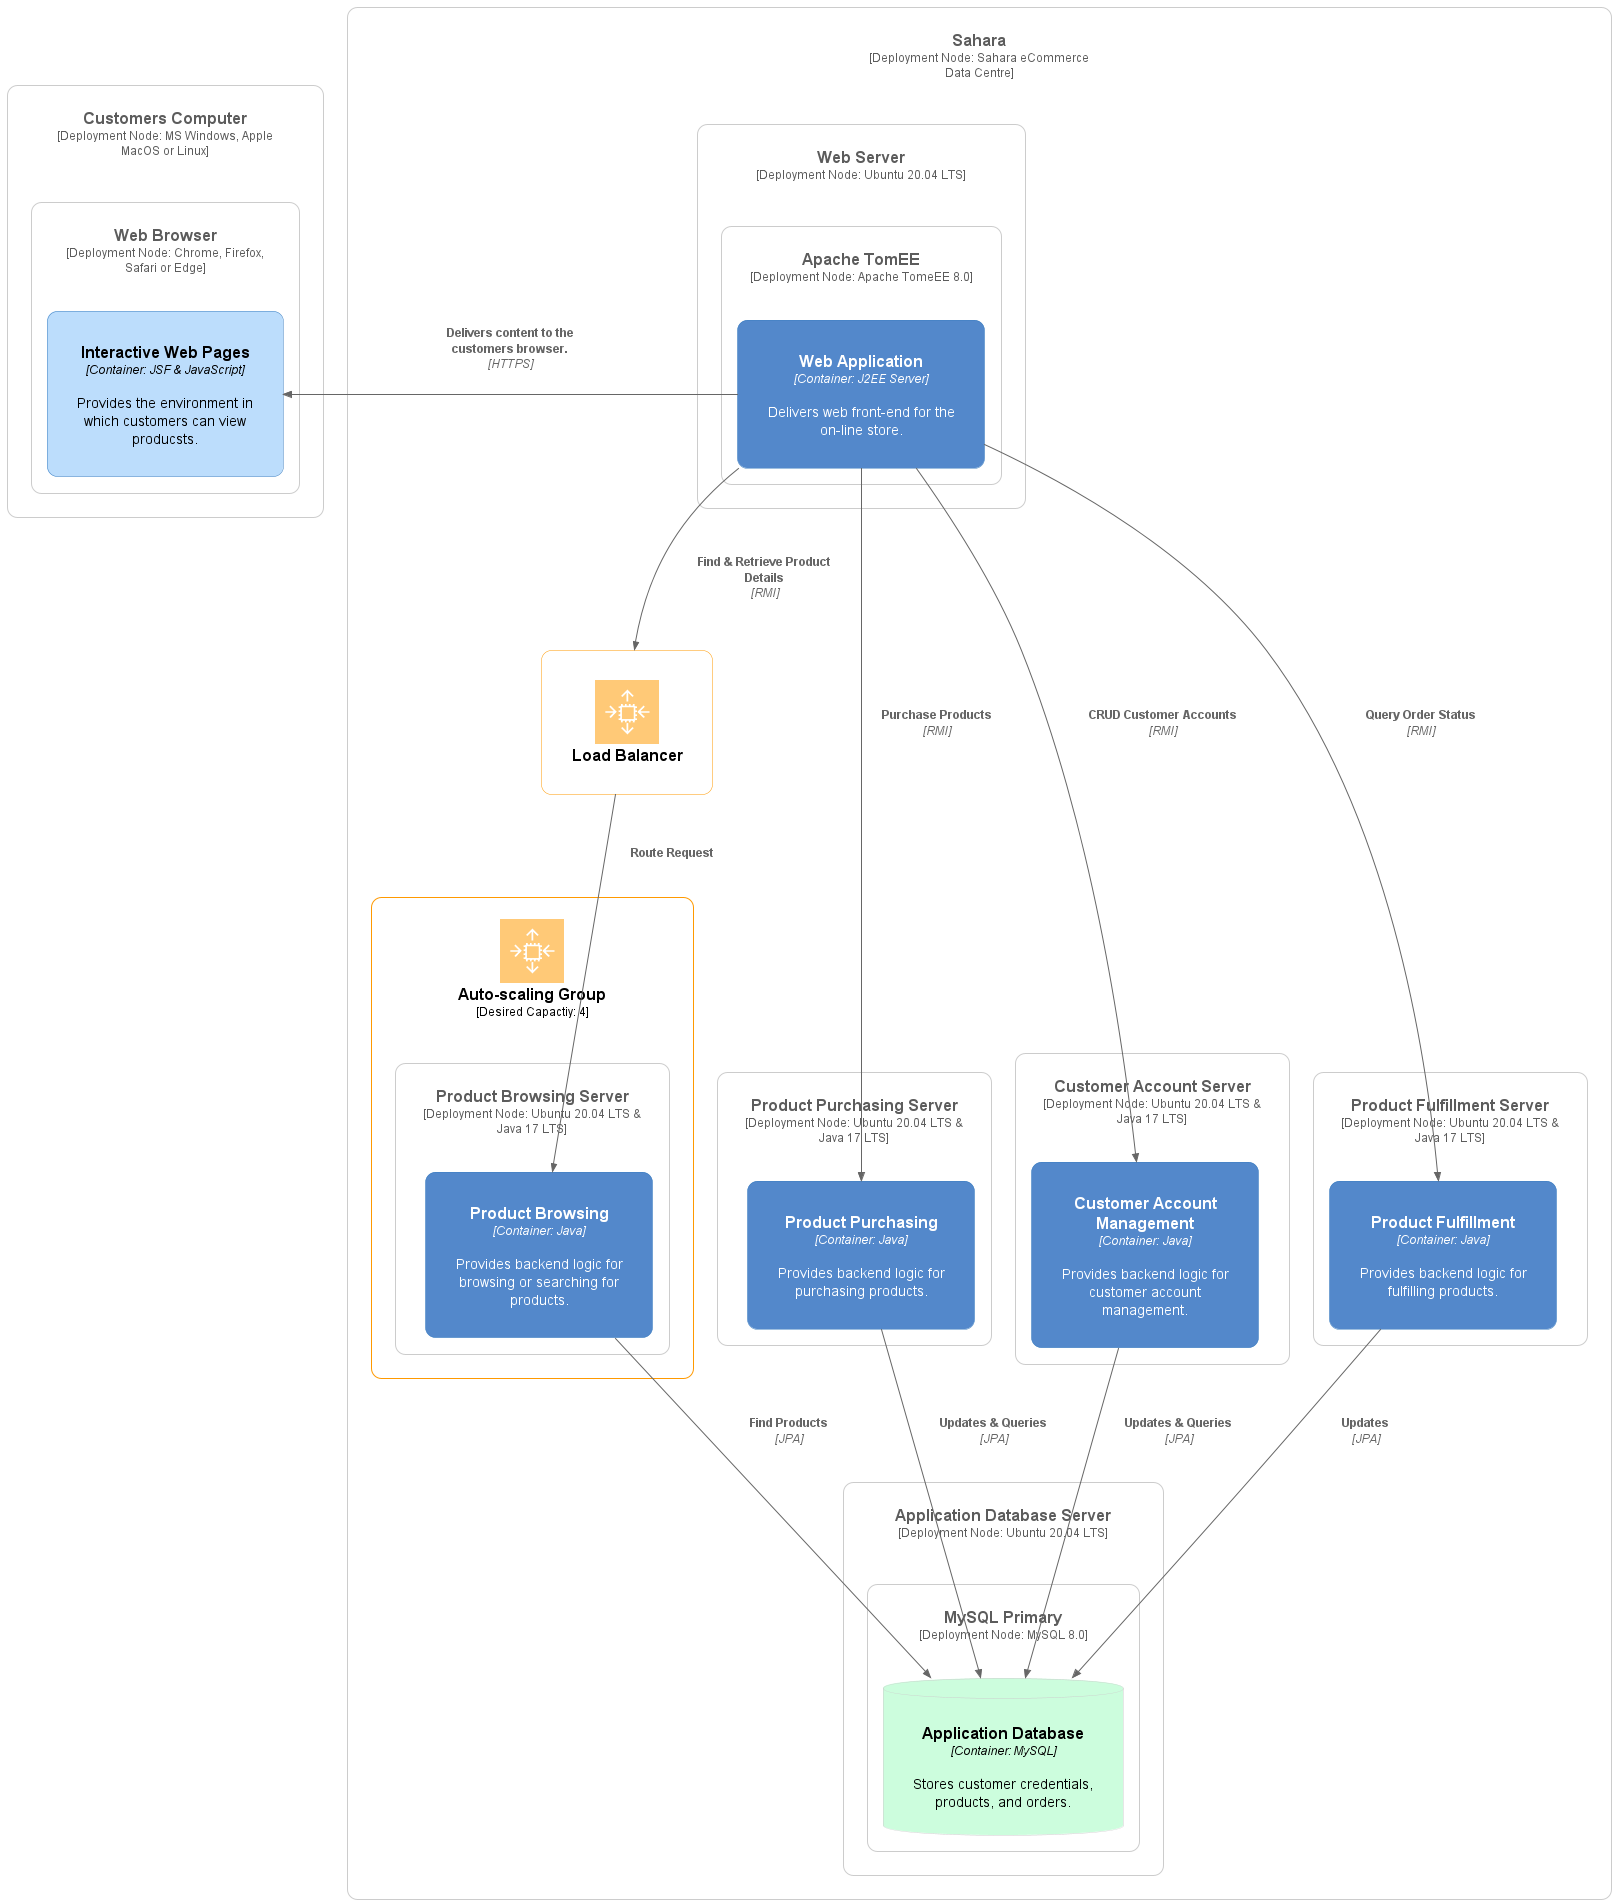
\includegraphics[width=0.8\textheight]{diagrams/SaharaScaled}
\end{center}
}

\question{What is the \highlight{problem}?}

\point[Database]{
\begin{center}
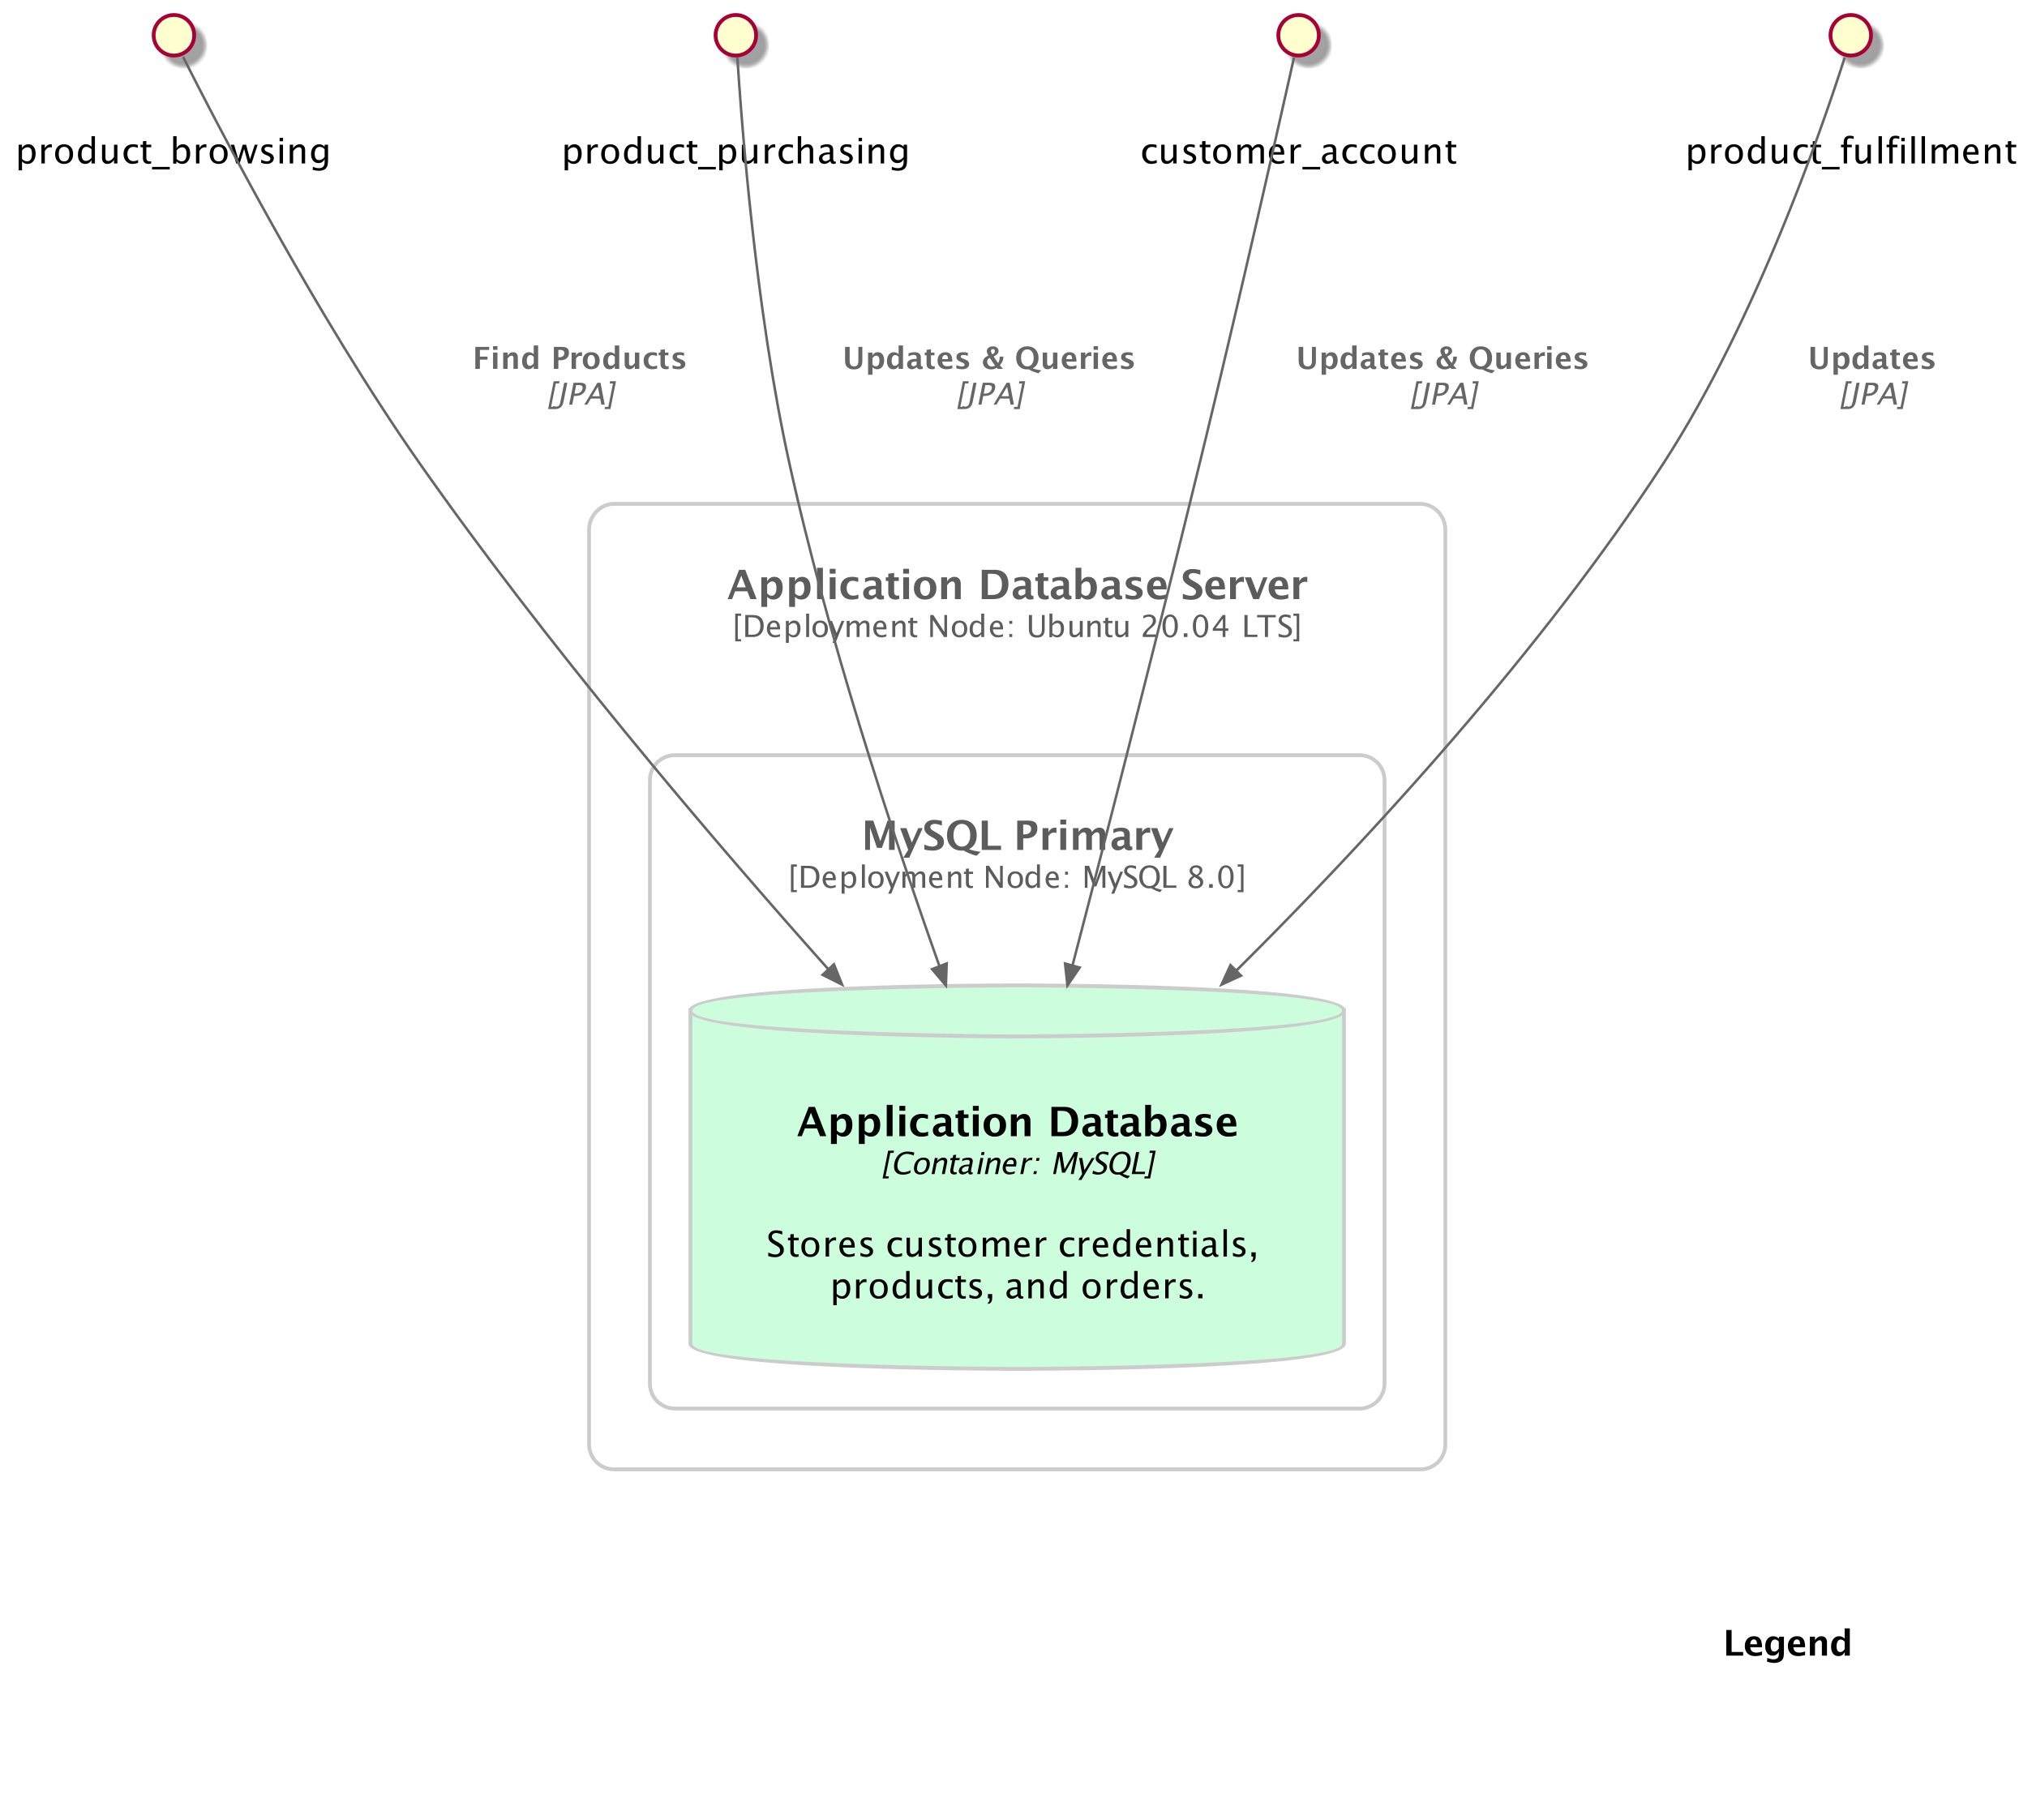
\includegraphics[width=\textheight]{diagrams/FocusDB}
\end{center}
}

\point[Disclaimer]{This is \highlight{not} a database course.}


%%%%%%%%%%%%%%%
% Replication %
%%%%%%%%%%%%%%%
\questionanswer{How do we fix database scaling issues?}{
    \begin{itemize}
        \item
        \only<3->{\highlight{Replication}}
        \only<-2>{Replication}
        \item Partitioning (or sharding)
        \item Independent databases
    \end{itemize}
}

\question{What is \highlight{replication}?}

\definition{Replication}{
    Data copied across multiple different machines.
}

\definition{Replica}{
    Database node which stores a copy of the data.
}


\questionanswer{What are the advantages of \highlight{replication}?}{
    \begin{itemize}[<+(1)->]
        \item Scale out our database to cope with load.
        \item Provide fault tolerance from a single database instance failure.
        \item Locate databases closer to end-users.
    \end{itemize}
}

\image{diagrams/LeaderFollower}

\point[Leader-based Replication]{
    \begin{description}[<+->]
        \item[On write] Writes sent to leader, change is propagated via change stream.
        \item[On read] Any replica can be queried. 
    \end{description}
}

\image{diagrams/LeaderFollowerSpread}

\point[Propogating changes]{
    \highlight{Synchronous} vs. \highlight{Asynchronous}
}

\point[Synchronous propagation]{
    Writes must propagate to \highlight{all followers} before being successful.
}

\point[Synchronous propagation]{
    \highlight{Any} replica goes down, \highlight{all} replicas are un-writable.
}

\point[Synchronous propagation]{
    Writes must \highlight{wait} for propagation to all replicas.
}

\point[Asynchronous propagation]{
    Writes \highlight{don't} have to \highlight{wait} for propagation.
}

\point[Asynchronous propagation]{
    If the leader goes down before propagating, the \highlight{write is lost}.
}

\point[Asynchronous propagation]{
    Replicas can have out-dated or \textsl{stale} data.
}

\todo{There could be content here about handling node failures}

% \point[When things go wrong]{
%     Handling outages
% }

% \point{Follower failure}

% \point{Leader failure}

\point[The time taken for replicas to update their stale data is]{Replication Lag}

\point[Eventually, all replicas must become consistent]{
    The system is \highlight{eventually consistent}
}

\point{Read-your-writes Consistency}

\point{Monotonic Reads}

\point{Consistent Prefix Reads}

\point{Solving Replication Lag}

\point{Multi-leader Replication}

\image[height=\textheight]{diagrams/MultiLeader}

\point[Multi-leader Replication]{Use Cases}

\note[itemize]{
    \item Multiple datacenters
    \item Offline writing
}

\point[Multi-leader Replication]{Problems}

\point[Parallel writes introduce]{Write conflicts}

\point[Where possible]{Avoid write conflicts}

\point[Where impossible]{Convergence}

\note[itemize]{
    \item Unique ID of writes
    \item Unique ID of replicas
    \item Simple merging strategies
    \item Explicit handling of conflicts
}

\point[Cutting Edge]{Automatic Conflict Resolution}

\point{Leaderless Replication}

\note[itemize]{Dynamo-style}

\image{diagrams/Leaderless}

\point[How are changes propagated?]{
    \begin{itemize}
        \item Read Repair
        \item Anti-entropy Process
    \end{itemize}
}

\questionanswer{How do a know it is consistent?}{Quorum Reads and Writes}

\todo{An example}

\definecolor{eq1}{RGB}{227, 206, 116}
\definecolor{eq2}{RGB}{227, 116, 137}

\point[Quorum Consistency]{
\begin{equation*}
\textcolor{eq1}{w} + \textcolor{eq2}{r} > \textcolor{focus}{n}
\end{equation*}
\Large
\begin{description}
    \item[$\textcolor{focus}{n}$] total replicas
    \item[$\textcolor{eq1}{w}$] amount of replicas to {\color{eq1}\textsl{write}} to
    \item[$\textcolor{eq2}{r}$] amount of replicas to {\color{eq2}\textsl{read}} from
\end{description}
}

%%%%%%%%%%%%%%%%
% Partitioning %
%%%%%%%%%%%%%%%%
\questionanswer{How do we fix database scaling issues?}{
    \begin{itemize}
        \item 
        \only<-2>{\highlight{Replication}}
        \only<3->{Replication}
        \item 
        \only<3->{\highlight{Partitioning (or sharding)}}
        \only<-2>{Partitioning (or sharding)}
        \item Independent databases
    \end{itemize}
}


%%%%%%%%%%%%%%%%%%%%%%%%%%%%%
% Isolation (foreshadowing) %
%%%%%%%%%%%%%%%%%%%%%%%%%%%%%
\questionanswer{How do we fix database scaling issues?}{
    \begin{itemize}
        \item Replication
        \item 
        \only<-2>{\highlight{Partitioning (or sharding)}}
        \only<3->{Partitioning (or sharding)}
        \item 
        \only<3->{\highlight{Independent databases}}
        \only<-2>{Independent databases}
    \end{itemize}
}

% \references{articles,books}

\end{document}